\documentclass[11pt, a4paper, oneside, openright]{article}

% Generelles Setup (Seitenränder) und Abstand zum Binden der Arbeit
\usepackage[dvips, bottom=4cm, top=3cm, right=3cm, left=3cm, bindingoffset=5mm]{geometry}



% Encoding (UTF8-Kompatabilität), Deutsche Sprache, Font-Encoding für Umlaute, Moderne Schrift
\usepackage[utf8]{inputenc}
\usepackage[ngerman]{babel}
\usepackage[T1]{fontenc}
\usepackage{lmodern}



% Schusterjungen und Hurdenkinder verhindern
\clubpenalty=10000
\widowpenalty=10000
\displaywidowpenalty=10000



% Anführungszeichen im dt. Stil, (unten 99, oben 66), Zitate mit \enquote{zitierter Text}
\usepackage[babel, german=quotes]{csquotes}



% Mathematik-Pakete
\usepackage{amssymb}
\usepackage{amsthm}
\usepackage{amsmath}
\usepackage[tbtags]{mathtools}
\usepackage{pgfplots}



% weitere Pakete (Optionen werden in eckigen Klammern geladen)
\usepackage{enumerate}
\usepackage{enumitem}
\usepackage{xspace}
\usepackage{graphicx}
\usepackage{pdfpages}
\usepackage{framed}
\usepackage{mdframed}
\usepackage{relsize}
\usepackage{float} 
\usepackage{pdfpages} 
\usepackage{longtable}
\usepackage[bottom]{footmisc}
\usepackage{lipsum}
\usepackage{blindtext}
\usepackage{calligra}
\usepackage[hyphenbreaks]{breakurl}
\usepackage{xurl}
\usepackage{microtype}



% Captions unter Bildern, Tabellen, Quelltexten etc. anpassen
\usepackage[font={scriptsize}, labelfont=bf, format=hang]{caption}
\usepackage[font={scriptsize}, labelfont=bf, labelformat=simple]{subcaption}
\renewcommand{\thesubfigure}{\,(\alph{subfigure})} 



% Pseudocode-Setup (in den eckigen Klammern)
\usepackage[linesnumbered, commentsnumbered, boxed, german]{algorithm2e}
\renewcommand{\listalgorithmcfname}{Algorithmenverzeichnis}



% Quelltexte einbinden, Namen ändern
\usepackage{listings}
\renewcommand{\lstlistingname}{Quelltext} 
\renewcommand{\lstlistlistingname}{Quelltextverzeichnis}



% Hyperref-Setup (Verweise sind verlinkt, sodass an die korrekte Stelle gesprungen wird)
\usepackage{hyperref}
\hypersetup{
    colorlinks,
    pdfpagelabels,
    pdfstartview = FitH,
    bookmarksopen = true,
    bookmarksnumbered = true,
    linkcolor = black,
    plainpages = false,
    hypertexnames = false,
    citecolor = black,
}



% Zeilenabstand
\usepackage{setspace}
\setstretch{1.5}


 
% PDF-Kompression ausstellen
\pdfcompresslevel=0
\pdfobjcompresslevel=0
\pdfimageresolution=4000



% Abkürzungen (sorgt für die typographisch-korrekten Abstände)
\newcommand \ggfs{ggfs.\xspace }
\newcommand \zB{z.\,B.\xspace }
\newcommand \sieheoben{s.\,o.\xspace }
\newcommand \siehe{s.\xspace }
\newcommand \dasheisst{d.\,h.\xspace }
\newcommand \ua{u.\,a.\xspace }
\newcommand \ia{i.\,a.\xspace }
\newcommand \idR{i.\,d.\,R.\xspace }
\newcommand \bspw{bspw.\xspace }
\newcommand \bzw{bzw.\xspace }
\newcommand \evtl{evtl.\xspace }
\newcommand \bzgl{bzgl.\xspace }
\newcommand \und{u.\xspace }
\newcommand \vgl{vgl.\xspace }
\newcommand \usw{u.\,s.\,w.\xspace }
\newcommand \insbes{insbes.\xspace }
\newcommand \etc{etc.\xspace }
\newcommand \sog{sog.\xspace }
\newcommand \ca{ca.\xspace }
\newcommand \zT{z.\,T.\xspace }
\newcommand \so{s.\,o.\xspace }
\newcommand \etal{et.\,al.\xspace }
\newcommand \ebd{ebd.\xspace }
\newcommand \ebdS{ebd.\,S.\,}
\newcommand \va{v.\,a.\xspace }
\newcommand \vglebd{vgl.\,ebd.\xspace }
\newcommand \vglebdS{vgl.\,ebd.\,S.\,}
\newcommand \Seite{S.\,}
\newcommand \Kap{Kap.\xspace }
\newcommand \Abb{Abb.\xspace }
\newcommand \jew{jew.\xspace }
\newcommand \versch{versch.\xspace }
\newcommand \engl{engl.\xspace }
\newcommand \EF{EF\xspace }
\newcommand \UVH{UVH\xspace }
\newcommand \Abs{Abs.\,}
\newcommand \wahrsch{wahrsch.\xspace }
\newcommand \Zeile{Z.\,}
\newcommand{\RM}[1]{\MakeUppercase{\romannumeral #1{}}}



% Farben (in RGB definiert)
\usepackage{xcolor}
\usepackage{colortbl}
\definecolor{dunkelgrau}{rgb}{0.75,0.75,0.75}
\definecolor{mittelgrau}{rgb}{0.85,0.85,0.85}
\definecolor{hellgrau}{rgb}{0.95,0.95,0.95}
\definecolor{deepblue}{rgb}{0,0,0.5}
\definecolor{deepred}{rgb}{0.6,0,0}
\definecolor{deepgreen}{rgb}{0,0.5,0}
\definecolor{bondiblue}{rgb}{0.0, 0.58, 0.71}
\definecolor{lightblue}{rgb}{0.68, 0.85, 0.9}
\definecolor{lightgreen}{rgb}{0.56, 0.93, 0.56}



% Quelltext-Umgebung fü Java definieren:
\newcommand\javastyle{\lstset{
    language=Java,
    otherkeywords={},
    keywordstyle=\color{deepblue},
    emph={},          
    emphstyle=\color{deepred},
    stringstyle=\color{deepgreen},
    commentstyle=\color{orange},    
    frame=,
    showstringspaces=false,
    showtabs=true,
    tabsize=3,
    tab=,
    showstringspaces=true,
    numbers=left,
    breakatwhitespace=true,
    breakatwhitespace = true,
    breakindent = 2ex,
    extendedchars=true,
    breaklines=true,
    numberstyle=\tiny,
    numbersep=9pt,
    stepnumber=1,
    captionpos=b,
    backgroundcolor=\color{hellgrau}
}}



% Zwei verschiedene Textgrößen definieren

% a) für den Fließtext
\newcommand\javastyleTextgroesseNormal{\lstset{
    basicstyle=\ttfamily\mdseries\color{black}\linespread{0.8}
}}

% b) für längere Zitate
\newcommand\javastyleTextgroesseKlein{\lstset{
    basicstyle=\scriptsize\ttfamily\mdseries\color{black}\linespread{0.8}
}}

% "Java" als neue Umgebung definieren
\lstnewenvironment{java}[1][]{\javastyle\javastyleTextgroesseKlein\lstset{#1}}{}

% Java-Umgebung für externe Dateien definieren
\newcommand\javaexternal[2][]{{\javastyle\javastyleTextgroesseKlein\lstinputlisting[#1]{#2}}}

% Java-Code im Fließtext
\newcommand\javainline[1]{{\javastyle\javastyleTextgroesseNormal\lstinline!#1!}}



% Titel und Autor
% Stichworte beim hyperref-Setup ändern!
\title{Der Sortieralgorithmus >>Quicksort<< und seine Implementation in Java mithilfe der\\ NRW-Landesklasse für die Datenstruktur Liste}
\author{Heiner Stroick}
\date{Version: \today}

\makeatletter
\hypersetup{
    pdftitle={\@title},
    pdfauthor={\@author},
    pdfsubject={Facharbeit, Quicksort, Liste, Algorithmus, Implementation} % hier Stichworte ändern
}
\makeatother



% ACHTUNG!
% Vor dem Ausdruck auskommentieren
% Das Paket kann helfen, Fehler in Verweisen aufzudecken
% \usepackage{refcheck}

% Das Paket kann helfen, zu lange Zeilen zu entdecken
% \usepackage{showframe}





%%%%%%%%%%%%%%%%%%%%%%%%%%%%%%%%
%%%%%%%                  %%%%%%%
%%%%%%%   ENDE PRÄAMEL   %%%%%%%
%%%%%%%                  %%%%%%%
%%%%%%%%%%%%%%%%%%%%%%%%%%%%%%%%





\begin{document}

\maketitle
\thispagestyle{empty}

\vfill

\noindent
\begin{tabular}{p{4cm}l}
    Fach:                   & Informatik \tabularnewline
    Kurs:                   & Q1 Grundkurs 1 \tabularnewline
    Betreuender Lehrer:     & Herr Stroick \tabularnewline
    Themenausgabe:          & 14. März 2021 \tabularnewline
    Abgabe:                 & 01. August 2021 \tabularnewline
\end{tabular}





\newpage
\setcounter{page}{1}
\pdfbookmark[1]{Inhaltsverzeichnis}{Inhaltsverzeichnis} 
\tableofcontents





\newpage
\section{Informationen zu dieser Mini-Facharbeit}
Diese \enquote{Mini-Facharbeit} dient zu Demonstrationszwecken und erhebt dabei  keinen Anspruch auf Vollständigkeit oder eine angemessene inhaltliche Tiefe. Sie soll den prinzipiellen Aufbau von Kapiteln anhand eines bekannten Beispiels verdeutlichen (nicht alle Kapitel sind vollständig ausformuliert, \vgl\zB\Kap\ref{sec:persoenlicherBezug}). Dabei wird zwischen >>Erklärung des Algorithmus<< und >>Implementation des Algorithmus<< unterschieden (\Kap\ref{sec:quicksort} und \Kap\ref{sec:implementation}).

Die \texttt{tex}-Datei kann dabei als Vorlage für die eigene Facharbeit dienen. Es wurde zudem versucht, verschiedene Möglichkeiten von Latex aufzuzeigen (\zB Aufzählungen, Stichwortlisten, Textauszeichnungen, Verweise, Zitate, Literaturverweise, eingebundene Bilder, Einbinden von Pseudocode und Quelltexten, \ldots), sodass die \texttt{tex}-Datei auch als Nachschlagewerk am praktischen Beispiel verstanden werden kann.

Für die eigene Facharbeit muss dann am Ende selbst entschieden werden, ob und wie die Reihenfolge der (Unter-)Kapitel vielleicht angepasst werden muss (\evtl ist auch nicht die Darstellung in der vorliegenden Kleinschrittigkeit sinnvoll). Gleiches gilt für die im Anhang aufgeführten Verzeichnisse (in dieser Facharbeit sind die Verzeichnisse aufgeführt, um die Möglichkeiten von Latex zu demonstrieren).

Diese Vorlage wurde unter \url{https://github.com/hnrstrck/vorlage_facharbeit} veröffentlicht. Das Datum auf der Titelseite entspricht der \enquote{Version} dieser Vorlage.

\vspace{1em}

\begin{center}
    \fontsize{20pt}{16pt}{\calligra{Viel Erfolg!}}
\end{center}

\vspace{1em}

\hfill\today~-- H. \textsc{Stroick}





\newpage
\section{Einleitung}
Sortierten Datenmengen begegnen wir jeden Tag: Sei es die nach Punkten sortierte Bundesligatabelle, die chronologisch sortierten E-Mails (mehrerer Accounts) in der Inbox oder die nach Namen sortierten Dateien in einem Ordner auf dem Computer. Das Zurechtfinden gelingt in sortierten Daten einfach besser als in Unsortierten.

Dabei ist das Herstellen von Ordnung -- das Sortieren an sich -- kein triviales Problem. In der Informatik wird versucht, unter Berücksichtigung verschiedener Zielvorgaben Sortieralgorithmen zu entwickeln und zu studieren. Häufig wird verlangt, dass Algorithmen unsortierte Daten (wie \bspw in \Abb\ref{fig:unsortierteDaten}) möglichst speicherplatzeffizient (so wenig RAM wie möglich nutzend), mit möglichst wenig Vertauschungen oder mit möglichst wenig Vergleichen zu sortieren. Zum Teil werden diese Anforderungen kombiniert.

\begin{figure}[H]
    \centering
    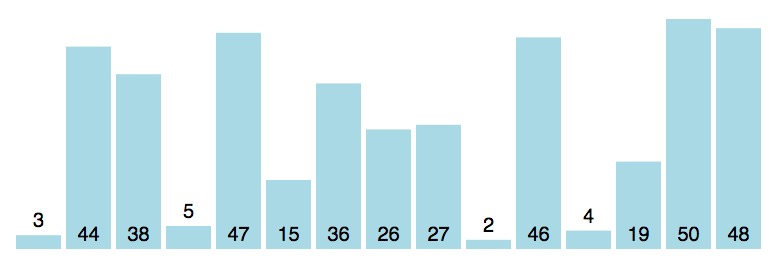
\includegraphics[width=12cm]{bilder/unsortierte_Daten.png}
    \caption[Unsortierte Daten.]{Unsortierte Daten. Bild: Screenshot von \cite{visualgoQS}.}
    \label{fig:unsortierteDaten}
\end{figure}

Es gibt eine Vielzahl an verschiedenen Sortieralgorithmen, die nach unterschiedlichen Prinzipien funktionieren. Beim Sortieren ist es allerdings unerheblich, ob lexikographisch, chronologisch oder direkt nach Zahlen sortiert wird. Durch Umrechnungen kann jedes Sortierproblem auf ein Sortierproblem von Zahlen zurückgeführt werden (\bspw durch den Einsatz des ASCII-Codes zum Umrechnen von Buchstaben in Zahlen).

Es sind \evtl auch noch andere Kriterien für die Wahl eines passenden Sortieralgoirthmus ausschlaggebend: Steht zu Beginn die Anzahl der zu sortierenden Daten noch nicht fest (weil die Daten \bspw nach und nach eintreffen), ist ein Algorithmus zu wählen, der nicht den \enquote{Überblick} über \emph{alle} Daten verlangt.

\begin{figure}[H]
    \centering
    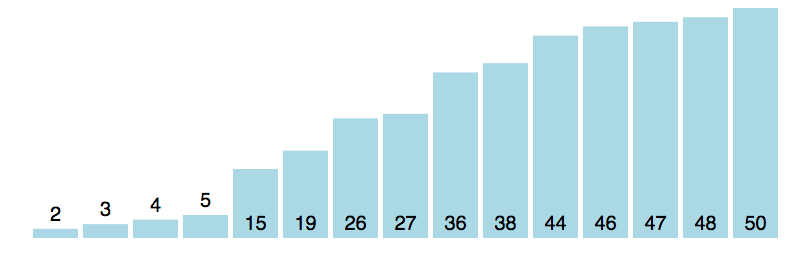
\includegraphics[width=12cm]{bilder/sortierte_Daten.png}
    \caption[Sortierte Daten.]{Sortierte Daten. Bild: Screenshot von \cite{visualgoQS}.}
    \label{fig:sortierteDaten}
\end{figure}

Ziel ist die korrekte Sortierung der Ausgangsdaten (wie in Abbildung \ref{fig:sortierteDaten} dargestellt). \cite{wikiSortierverfahren} gibt einen guten Überblick über verschiedene Sortierverfahren. Die dort veröffentlichte Tabelle zeigt auch sehr schön, wie sich verschiedene Algorithmen in ihren Laufzeiten unterscheiden, \dasheisst wie \enquote{schnell} oder \enquote{langsam} sie eine Menge von $n$ Zahlen sortieren (dafür wird die \sog $\mathcal{O}$-Notation\footnote{Informationen: Linux Related (2014): \emph{Laufzeitkomplexität von Algorithmen -- die O-Notation}, \url{http://www.linux-related.de/index.html?/coding/o-notation.htm}, besucht am 09.04.2020.} verwendet).





\subsection{Historie des Quicksort-Algorithmus}
Der Quicksort-Algorithmus wurde von Tony \textsc{Hoare}\footnote{\enquote{Sir Charles Antony Richard \textsc{Hoare} (* 11.~Januar 1934 in Colombo, Sri Lanka), besser bekannt als Tony \textsc{Hoare} oder C.A.R.~\textsc{Hoare}, ist ein britischer Informatiker. \textsc{Hoare} erlangte hohes Ansehen durch die Entwicklung des Quicksort-Algorithmus sowie des \textsc{Hoare}-Kalküls, durch den sich die Korrektheit von Algorithmen beweisen lässt.} \cite{wikiHoare}} entwickelt und 1962 in \cite{hoare} erstmalig vorgestellt und analysiert. Quicksort ist ein Algorithmus, der sich insbesondere durch seine Geschwindigkeit, seine effektive Speicherplatznutzung und seine simple Programmierung auszeichnet (\enquote{The method compares very favourably with other known methods in speed, in economy of storage, and in ease of programming}, \cite[\Seite 1]{hoare}). Seit seiner Veröffentlichung wurde der Algorithmus von vielen Informatikern analysiert und verbessert (\vgl\cite{wikiQS}).





\subsection{Divide and Conquer}
Quicksort setzt die Divide-and-Conquer-Strategie (auch D\&C, >>Teile und Herrsche<<) zum Sortieren ein. Eine Erklärung dieser Strategie wird von \textsc{Hoare} in seinem Paper gegeben (\vgl \cite[\Seite 1]{hoare}); an dieser Stelle sei der Einfachheit halber auf die in \cite{uniflensburgDuC} aufgeführten Erläuterungen verwiesen. Ein Lösungsansatz, der nach dem Divide-and-Conquer-Prinzip arbeitet, gliedert sich immer in dieselben drei Schritte:

\begin{table}[H]
    \begin{center}
        \begin{tabular}{p{2cm}p{10cm}}
            \textbf{Divide}  & Das Problem wird in Teilprobleme zerlegt. \\
            \textbf{Conquer} & Die Teilprobleme werden gelöst. \\
            \textbf{Combine} & Die Lösungen der Teilprobleme werden zusammengefügt, so dass sie die Lösung des ursprünglichen Problems ergeben.
        \end{tabular} 
        \caption[Schritte der Divide-and-Conquer-Strategie.]{Die Schritte der Divide-and-Conquer-Strategie zur Lösung eines Problems nach \cite{uniflensburgDuC}.}
        \label{tabl:dundc}
    \end{center}
\end{table}

Quicksort setzt die Divide-and-Conquer-Strategie sehr geschickt ein, um Daten zu sortieren. Dies wird in Kapitel~\ref{sec:ideeQuicksort} erläutert.





\subsection{Persönlicher Bezug zum Thema}
\label{sec:persoenlicherBezug}
\lipsum[1]{}





\subsection{Aufbau der Facharbeit}
In Kapitel~\ref{sec:quicksort} wird der Quicksort-Algorithmus in seiner Theorie vorgestellt. Nachdem die Idee des Algorithmus in Kapitel~\ref{sec:ideeQuicksort} erläutert wurde, wird die Laufzeit von Quicksort in Kapitel~\ref{sec:laufzeitQuicksort} in den Blick genommen. 

Kapitel~\ref{sec:implementation} widmet sich der Implementation. Da für die Programmierung in Java die NRW-Landesklasse \javainline{List} verwendet, wird diese zunächst vorgestellt (\Kap\ref{sec:landesklasseList}). Die anderen Klassen des Projekts werden in Kapitel~\ref{sec:andereKlassen} erläutert; das Klassendiagramm in Kapitel~\ref{sec:klassendiagramm} verschafft einen Überblick. Nach der Formulierung von des Quelltextes in Pseudocode (\Kap\ref{sec:pseudocodeQuicksort}) wird der eigentliche Java-Quelltext kleinschrittig erklärt (\Kap\ref{sec:quelltexterklaerung}). Zum Teil wird an bekanntes Wissen aus dem Unterricht angeknüpft.

Das Fazit in Kapitel~\ref{sec:fazit} fasst die Erkenntnisse dieser Facharbeit noch einmal zusammen und gibt einen Ausblick, der auch andere Sortierverfahren umfasst (Mergesort, Heapsort).

Kapitel~\ref{sec:weitereInfos} gibt Tipps zum Umgang mit Latex und zum Erstellen einer Facharbeit (\ua auch zur Literaturrecherche). Es wird außerdem auf hilfreiche Programme verwiesen, \bspw zum Erstellen von Grafiken / Zeichnungen, UML-Diagrammen oder Plotten von Funktionsgraphen (für eine Facharbeit in Mathematik).





\newpage
\section{Der Quicksort-Algorithmus}
\label{sec:quicksort}





\subsection{Idee des Algorithmus}
\label{sec:ideeQuicksort}
Ausgangspunkt ist eine Menge an zu sortierenden Elementen. Zuerst wird ein Element, das \emph{Trennelement} oder \emph{Pivotelement}\footnote{fraz. \emph{pivot} (Drehpunkt)}, bestimmt. Dann werden alle Elemente mit diesem Pivotelement nacheinander verglichen. Sind Elemente kleiner als das Pivotelement, kommen sie auf die linke Seite, sind sie größer als das Pivotelement, kommen sie auf die rechte Seite. Nun ist offenkundig, dass sich das Pivotelement schon an der richtigen Position befindet und an seiner Position sortiert vorliegt. Dann wird dieses Vorgehen auf die linke bzw. rechte Seite (mehrfach) rekursiv angewendet. Das Verfahren hört auf, wenn nur noch einelementige Mengen vorliegen (\vgl \cite{hoare}\cite{wikiQS}).

Die Idee wird in \cite{uniflensburgQS} etwas formaler vorgestellt: 

\begin{quote}
Zunächst wird die zu sortierende Folge $a$ so in zwei Teilstücke $b$ und $c$ zerlegt, dass alle Elemente des ersten Stücks $b$ kleiner oder gleich allen Elementen des zweiten Stücks $c$ sind (\emph{divide}). Danach werden die beiden Teilstücke sortiert, und zwar rekursiv nach demselben Verfahren (\emph{conquer}). Wieder zusammengesetzt ergeben die Teilstücke die sortierte Folge (\emph{combine}).

\hfill\cite{uniflensburgQS}
\end{quote}

Quicksort ist ein nicht-stabiles Sortierverfahren (\vgl \cite{wikiQS} und \cite{wikiStabilitaet}). Das bedeutet, dass sich die Reihenfolge von Datensätzen ändern kann, wenn nach verschiedenen Sortierschlüsseln sortiert wird. Beispiele finden sich unter \cite{wikiStabilitaet}.

Die Idee von Quicksort kann auch nonverbal dargestellt werden. Folgende Anleitung~\ref{fig:kvicksoert} ist im Stil eines großen schwedischen Möbelhauses gehalten und kommt ohne weitere Erklärungen aus. 

\begin{figure}[H]
    \centering
    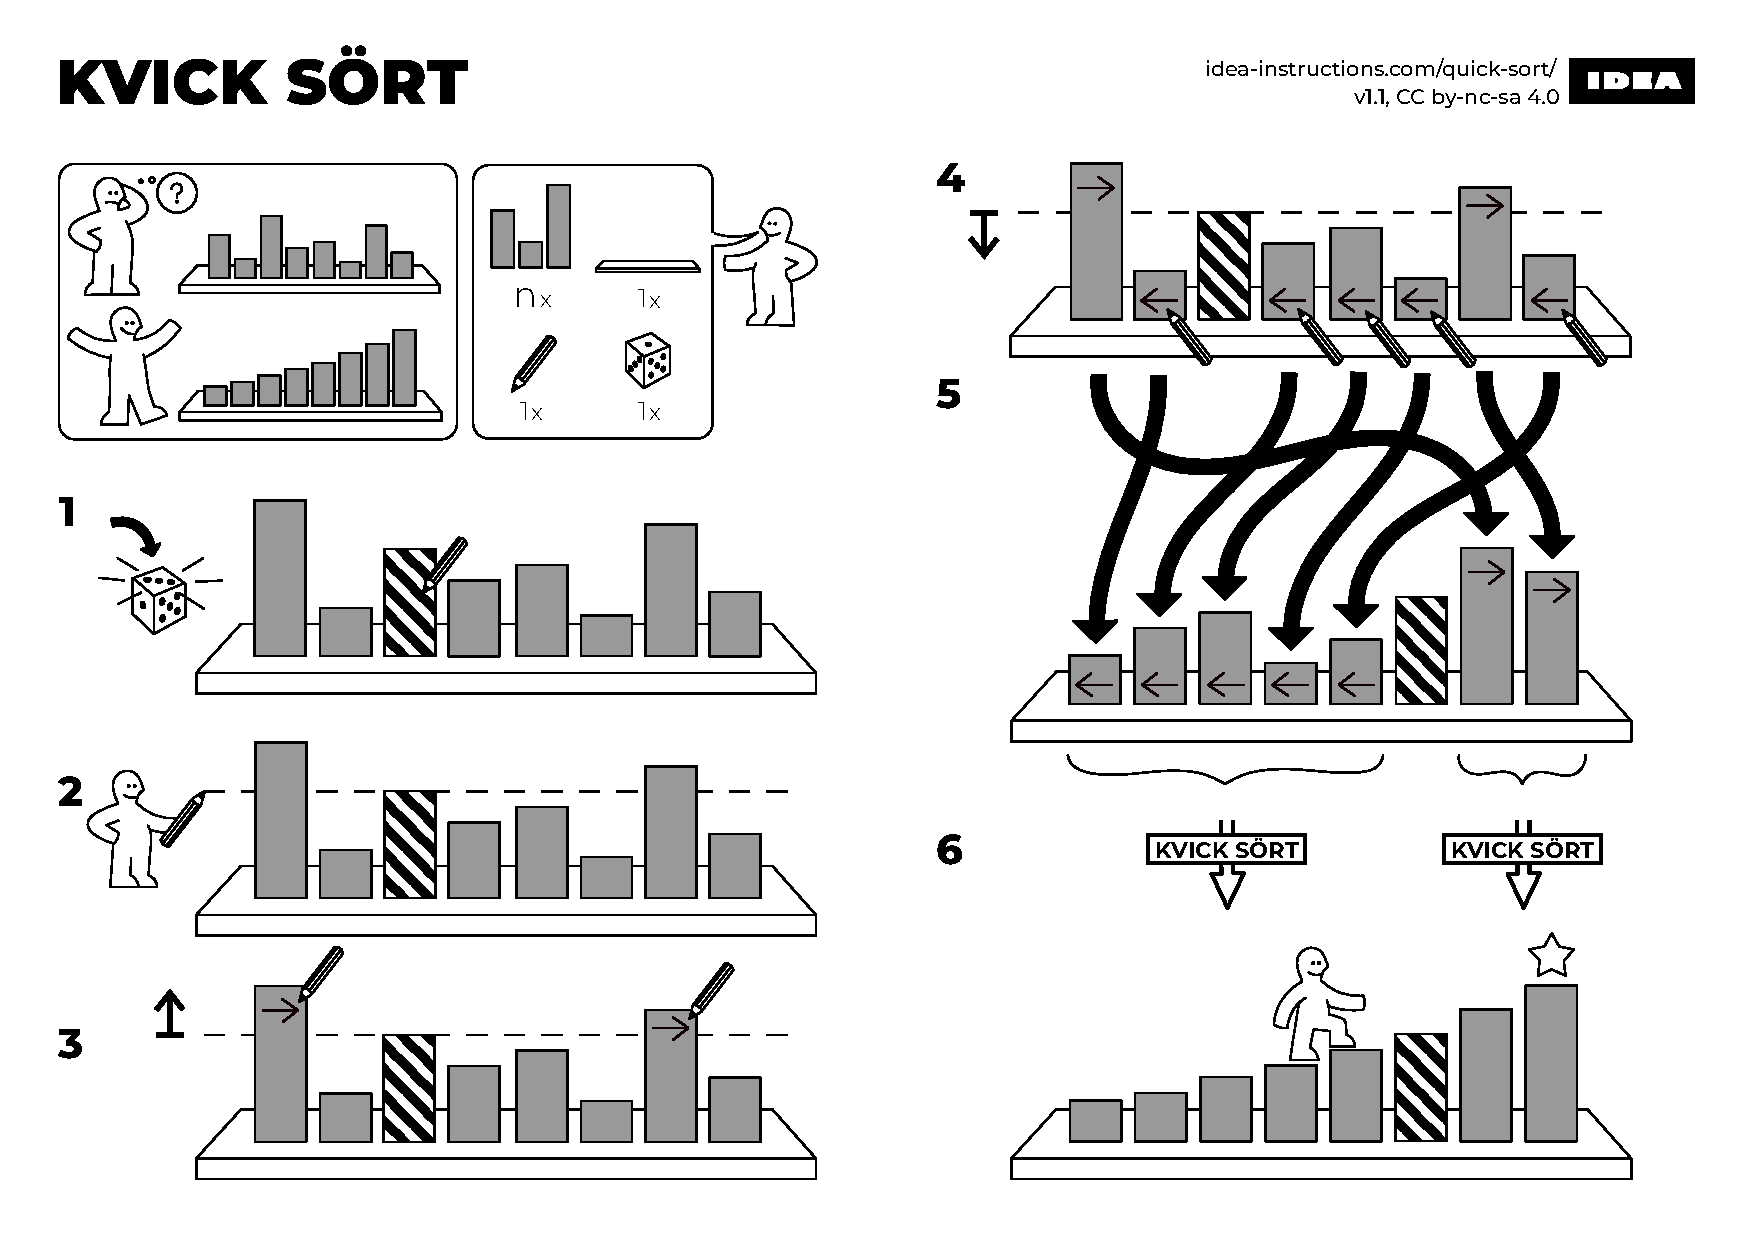
\includegraphics[width=\textwidth]{bilder/kvicksoert.pdf}
    \caption[Bildliche Darstellung des Quicksort-Algorithmus.]{Der Ablauf des Quicksort-Algorithmus als Bauanleitung >>\MakeUppercase{Kvick Sört}<<. Bild:~\cite{ideaBauanleitung}}
    \label{fig:kvicksoert}
\end{figure}





\subsection{Laufzeit}
\label{sec:laufzeitQuicksort}
Bei der Bewertung der Laufzeit von Quicksort ist die Problemgröße die Anzahl der zu sortierenden Zahlen -- offensichtlich steigt die Laufzeit, wenn mehr Zahlen zu sortieren sind. Die Problemgröße wird mit $n$ bezeichnet.  

Entscheidend für die Geschwindigkeit, mit der eine Datenmenge sortiert wird, ist die Wahl eines passenden Pivotelements, wie die folgenden Kapitel zeigen werden.





\subsubsection{Best-Case}
Im besten Falle trennt das Pivotelement die Liste genau so, dass linke rechte Liste gleichgroß sind, also gleichviele Elemente enthalten. Damit wird die geringste Rekursionstiefe erreicht (\vgl\Abb\ref{fig:darstellungQSbestcase}). 

Natürlich ist hier die Schwierigkeit, das Pivotelement entsprechend zu bestimmen. Statistische Verfahren können genutzt werden, um möglichst effizient ein entsprechendes Pivotelement zu ermitteln (\zB mit der Bestimmung eines Medians).

\begin{figure}[H]
    \centering
    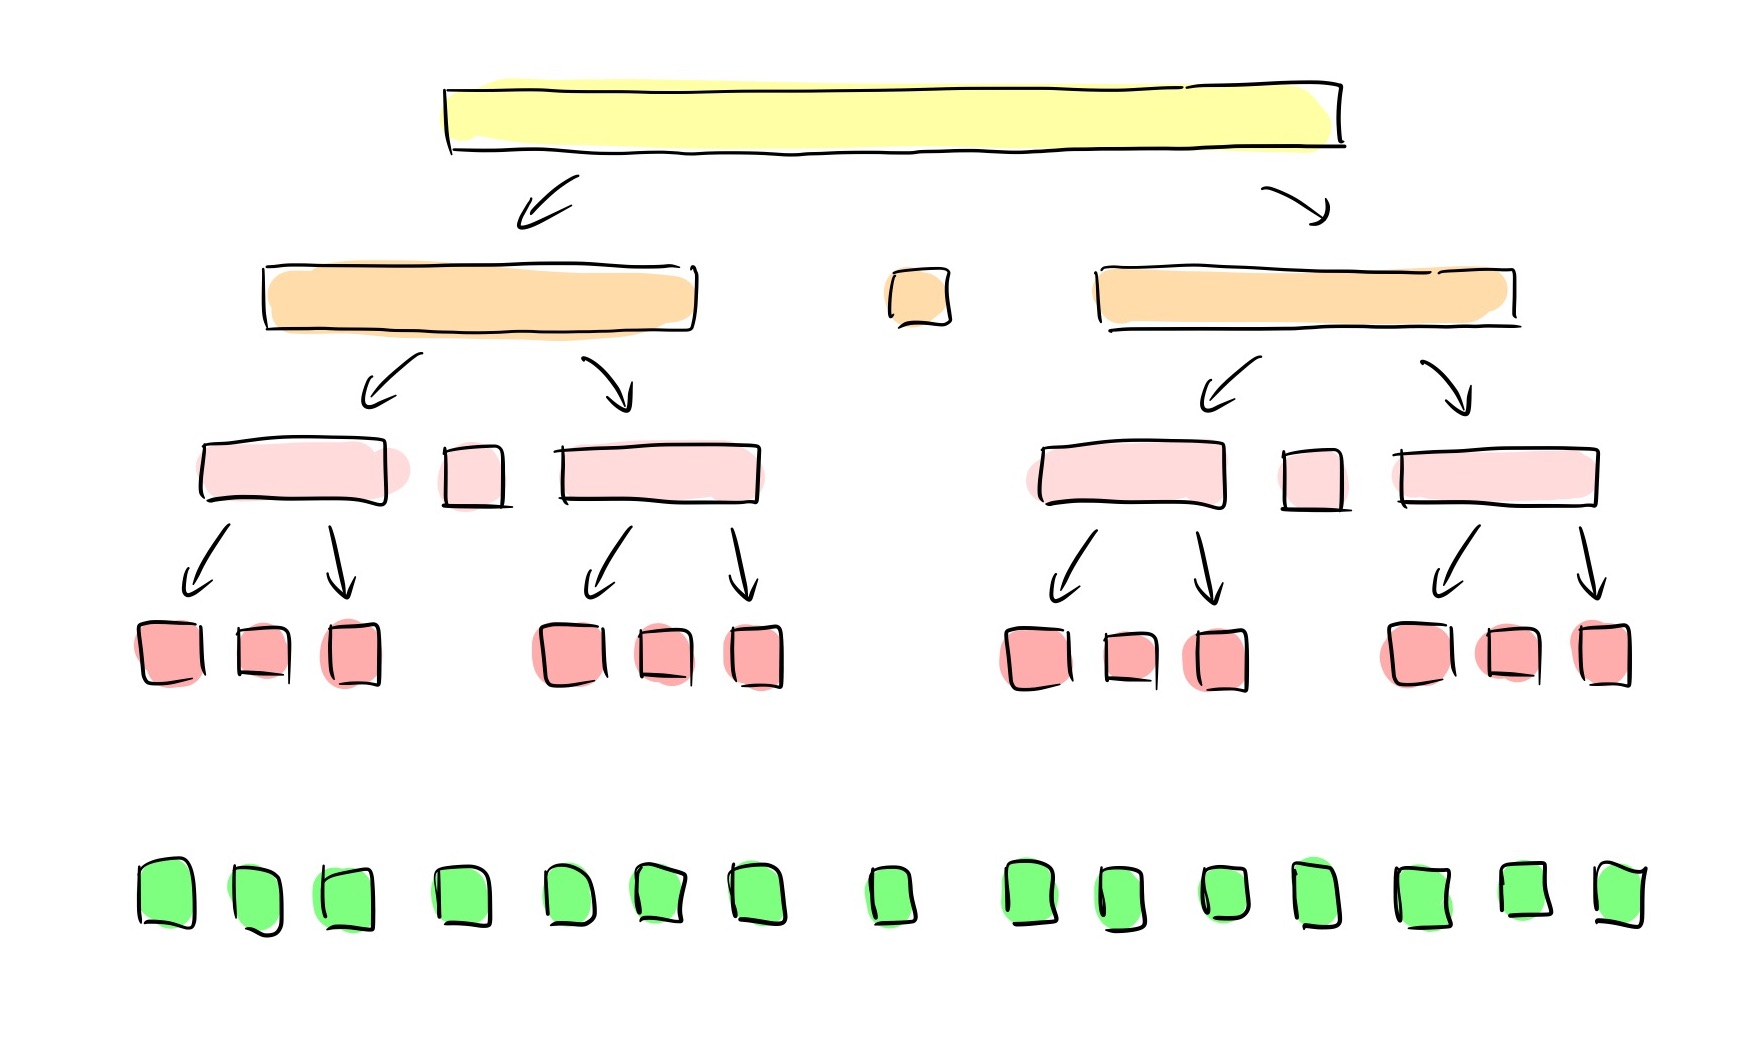
\includegraphics[width=12cm]{bilder/qs_bestcase.jpg}
    \caption[Darstellung der Rekursion im Best-Case.]{Das Pivotelement trennt eine Liste stets in zwei gleichgroße linke und rechte Listen. Dadurch bleibt die Rekursionstiefe minimal -- hier wird nur eine Rekursionstiefe von $t = 3$ erreicht.}
    \label{fig:darstellungQSbestcase}
\end{figure}

Es ergibt sich im besten Falle eine Laufzeit von 
$$\mathcal{O}\left(n \cdot \log_2{(n)}\right),$$
genaugenommen sogar von $\Theta\left(n \cdot \log_2{(n)}\right)$. Auf einen Beweis wird hier verzichtet.\footnote{Hinweis: In einer echten Facharbeit wäre dieser aber zu führen. Wie dies aussehen könnte, wird in \cite{khanqslaufzeit} deutlich.}  





\subsubsection{Worst-Case}
Im schlechtesten Fall wird in jedem Quicksort-Aufruf immer das größte (oder kleinste) Element als Pivotelement ausgewählt, sodass beim Aufteilen in linke und rechte Liste eine von beiden leer ist (dies kann auch bspw. abwechselnd passieren). Dadurch wird die maximale Rekursionstiefe erreicht. Dies ist insbesondere dann der Fall, wenn die zu sortierenden Daten schon sortiert vorliegen (und als Pivotelement immer das erste oder letzte Element gewählt wird).

\begin{figure}[H]
    \centering
    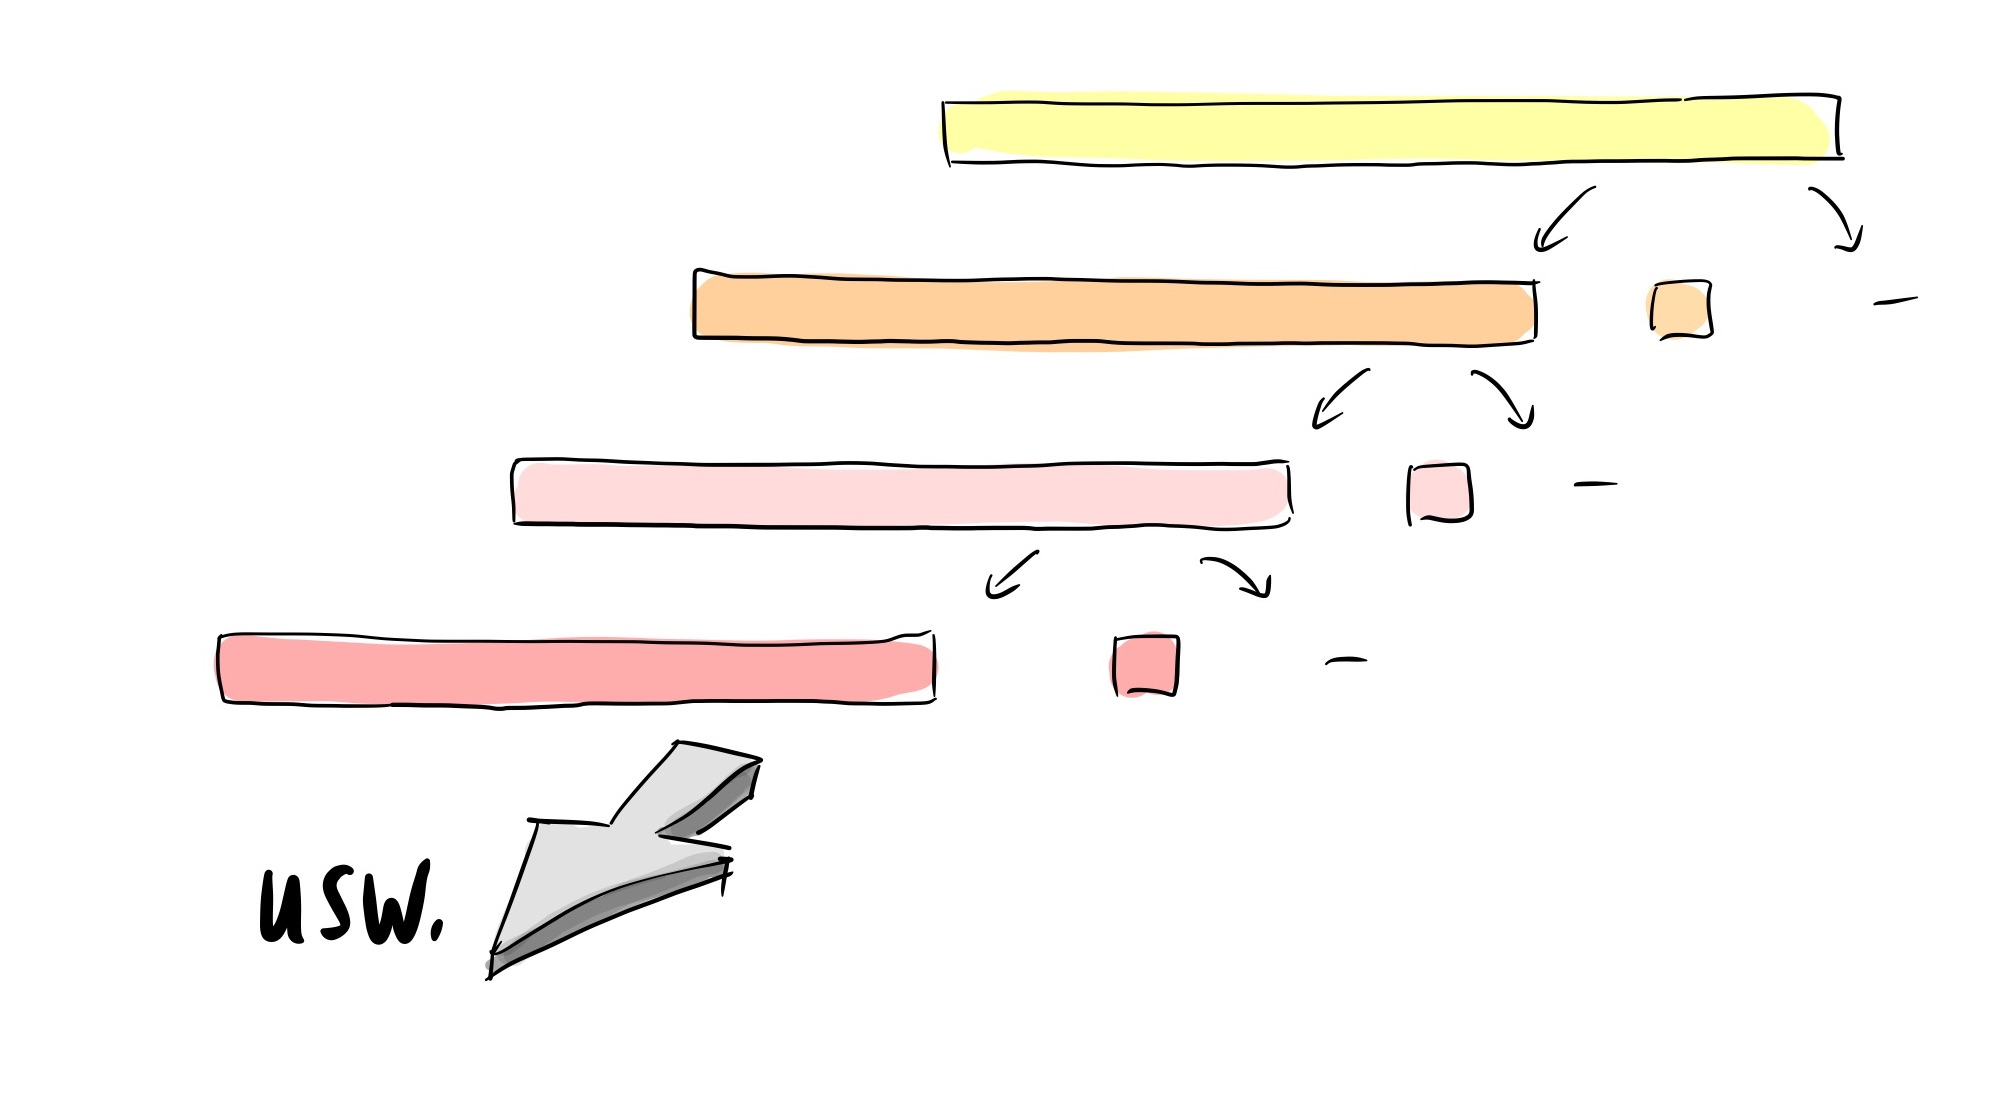
\includegraphics[width=12cm]{bilder/qs_worstcase.jpg}
    \caption[Darstellung der Rekursion im Worst-Case.]{Entwicklung der Rekursion im schlechtesten Fall. Das Pivotelement trennt die Listen so, dass eine Seite immer leer bleibt. Dabei ist natürlich unerheblich, ob \emph{immer} die rechte Liste leer bleibt oder ob dies abwechselnd (links und rechts) passiert. Es wird mit $t = 14$ die maximale Rekursionstiefe erreicht.}
    \label{fig:raspberry_logo}
\end{figure}

Es ergibt sich nach \cite[\Seite 119]{schoeninghQ1Q2} dabei der Wert 

\begin{equation}
(n-1) + (n-2) + \ldots + 4 + 3 + 2 = \frac{1}{2}n(n-1)-1 \label{eq:summeworstcase}
\end{equation}

für die Anzahl der Vergleiche. Die Laufzeit ist also quadratisch, also entsprechend $\Theta\left(n^2\right)$, da die Anzahl an Vergleichen den Zeitaufwand für das Sortieren im Wesentlichen bestimmt. In \cite{khanqslaufzeit} wird dies weiter ausgeführt.

Diese Summe aus \eqref{eq:summeworstcase} kann durch Anwenden der \textsc{Gauß}'schen Summenformel 

\begin{equation}
1 + 2 + 3 + \ldots + n = \sum_{k=1}^n k = \frac{1}{2}n(n+1) \tag{\textsc{Gauss}}\label{sec:gaussSummenformel}
\end{equation}

vereinfacht werden. Auf einen Beweis der Formel \eqref{sec:gaussSummenformel} wird hier aber verzichtet.





\subsubsection{Average-Case}
Ein intuitiver \enquote{Beweis} der mittleren Laufzeit wird bspw. bei \cite{khanqslaufzeit} gegeben. Auf eine weitere Darstellung wird an dieser Stelle aus Gründen des Umfangs verzichtet. Im mittleren Fall erreicht Quicksort ebenfalls eine Laufzeit von $\Theta\left(n \cdot \log_2{(n)}\right)$.





\subsubsection{Praxisrelevanz}
Es wird deutlich, dass die Wahl des Pivotelements entscheidenden Einfluss auf die Laufzeit hat. Die Wahrscheinlichkeit des Eintreffens des Worst-Case ist bei verschiedenen Ansätzen zur Bestimmung günstiger Pivotelemente unterschiedlich groß (Aufzählung nach \cite{wikiQS}):

\begin{itemize}

    \item \textbf{Naiver Ansatz}: Als Pivotlement wird immer das erste, letzte oder mittlere Element der Liste gewählt. Dieser naive Ansatz ist aber relativ ineffizient. 

    \item \textbf{Median-Ansatz}: Eine andere Möglichkeit ist es den Median dieser drei Elemente zu bestimmen und als Pivotelement zu verwenden. 

    \item \textbf{Randomisierter Quicksort}: Ein anderer Ansatz ist, als Pivotelement ein zufälliges Element auszuwählen. Bei diesem randomisierten Quicksort ist die Wahrscheinlichkeit, dass das Pivotelement in jedem Teilungsschritt so gewählt wird, dass sich die Worst-Case-Laufzeit ergibt, extrem gering. Man kann davon ausgehen, dass er praktisch nie auftritt.

    \item \textbf{Quicksort mit dem Median-of-medians-Algorithmus}: Verwendet man für die Wahl des Pivotelemts den Median-of-medians-Algorithmus, welcher den Median eines Arrays in $\mathcal{O}(n)$  bestimmt, so kann insgesamt eine Laufzeit von $\mathcal{O}\left(n\cdot \log_2{(n)}\right)$ für den schlechtesten Fall von Quicksort garantiert werden (\vgl auch \cite[\Kap\enquote{Analyse}]{uniflensburgQS}).

\end{itemize}





\subsubsection{Untere Schranke für vergleichsbasierte Sortierverfahren}
Quicksort einer der schnellsten Sortieralgorithmen, die es gibt (und geben kann!). Eine Erklärung dieser Tatsache wird in \cite[\Kap\enquote{Beweis der unteren Schranke für vergleichsbasiertes Sortieren}]{wikiSortierverfahren} gegeben, aber hier nicht weiter ausgeführt. Trotzdem soll sie in folgendem Theorem gewürdigt werden:

\begin{figure}[H]
    \begin{mdframed}[backgroundcolor=white, shadow=true, shadowcolor=dunkelgrau, linewidth=1pt, linecolor=deepred, shadowsize=3pt]
        {\small
            Es ist für ein vergleichsbasiertes Sortierverfahren nicht möglich, $n$ Zahlen schneller als in einer Zeit von $\mathcal{O}\left(n \cdot \log_2{(n)}\right)$ zu sortieren.

            $\Omega\left(n \cdot \log_2{(n)}\right)$ ist also die untere Laufzeitgrenze für vergleichsbasiertes Sortieren von $n$ Zahlen.
        }
    \end{mdframed}
\end{figure}





\subsection{Speicherplatz}
\label{sec:speicherplatzQuicksort}
Das Verwenden der Rekursion kostet Speicherplatz. In der Praxis wird es daher häufig so gehandhabt, dass die Rekursion des Quicksort-Algorithmus nur bis zu einer gewissen Tiefe angewendet und die restlichen Teillisten dann iterativ sortiert werden. Es gibt Varianten von Quicksort, die eine Rekursionstiefe von maximal $\log_2{(n)}$ garantieren (\vgl\bspw\cite{wikiQS}).





\newpage
\section{Implementation}
\label{sec:implementation}
Im Folgenden wird der QuickSort-Algorithmus mithilfe der NRW-Landesklasse \javainline{List} implementiert. Dafür werden die in Tabelle~\ref{tabl:staedtekreisborken} gegebenen Städte des Kreises Borken betrachtet, die nach ihrer Zahl der Einwohner sortiert werden sollen. Es wird also ein >>Städteranking<< gemessen an den Einwohnerzahlen erstellt.

\begin{table}[H]
    \begin{center}
        \begin{tabular}{|p{2.5cm}|p{3.5cm}|}

            \hline

            \rowcolor{blue!25}
            \textbf{Name} & \textbf{Einwohnerzahl} \\

            \hline
            \hline
            
            \texttt{Ahaus} & \texttt{39185} \\
            \texttt{Bocholt} & \texttt{71036} \\
            \texttt{Borken} & \texttt{42509} \\
            \texttt{Gescher} & \texttt{17253} \\
            \texttt{Gronau} & \texttt{47671} \\
            \texttt{Isselburg} & \texttt{10713} \\
            \texttt{Rhede} & \texttt{19165} \\
            \texttt{Stadtlohn} & \texttt{20367} \\
            \texttt{Velen} & \texttt{12989} \\
            \texttt{Vreden} & \texttt{22561} \\

            \hline

        \end{tabular} 
        \caption[Städte des Städterankings.]{Städte des Kreises Borken.}
        \label{tabl:staedtekreisborken}
    \end{center}
\end{table}





\subsection{Die generische Landesklasse \texttt{List}}
\label{sec:landesklasseList}
\enquote{Objekte der generischen Klasse \javainline{List} verwalten beliebig viele, linear angeordnete Objekte vom Typ \javainline{ContentType}. Auf höchstens ein Listenobjekt, aktuelles Objekt genannt, kann jeweils zugegriffen werden. Wenn eine Liste leer ist, vollständig durchlaufen wurde oder das aktuelle Objekt am Ende der Liste gelöscht wurde, gibt es kein aktuelles Objekt. Das erste oder das letzte Objekt einer Liste können durch einen Auftrag zum aktuellen Objekt gemacht werden. Außerdem kann das dem aktuellen Objekt folgende Listenobjekt zum neuen aktuellen Objekt werden. Das aktuelle Objekt kann gelesen, verändert oder gelöscht werden. Außerdem kann vor dem aktuellen Objekt ein Listenobjekt eingefügt werden.} \cite{lehrplannavigatorIFDokuGK} 

Die genauen Methodenbezeichnungen -- mitsamt Erläuterungen -- können im Anhang nachgeschlagen werden (Anhang \Seite\pageref{app:javadocliste}). Die Landesklasse \javainline{List} kann auf der Materialseite für Informatik (\enquote{Lehrplannavigator}) unter \cite[\Abs\enquote{Grundlegende Materialien und Dokumentationen für den Unterricht und für das Zentralabitur}]{lehrplannavigatorIF} heruntergeladen werden (ebenfalls sind dort die Landesklassen für die anderen Datenstrukturen veröffentlicht).





\subsection{Andere Klassen des Projekts}
\label{sec:andereKlassen}
Abbildung~\ref{fig:bluejscreenshot} zeigt das BlueJ-Projekt und die übrigen Klassen, deren Funktionen im Folgenden erläutert werden.

\begin{figure}[H]
    \centering
    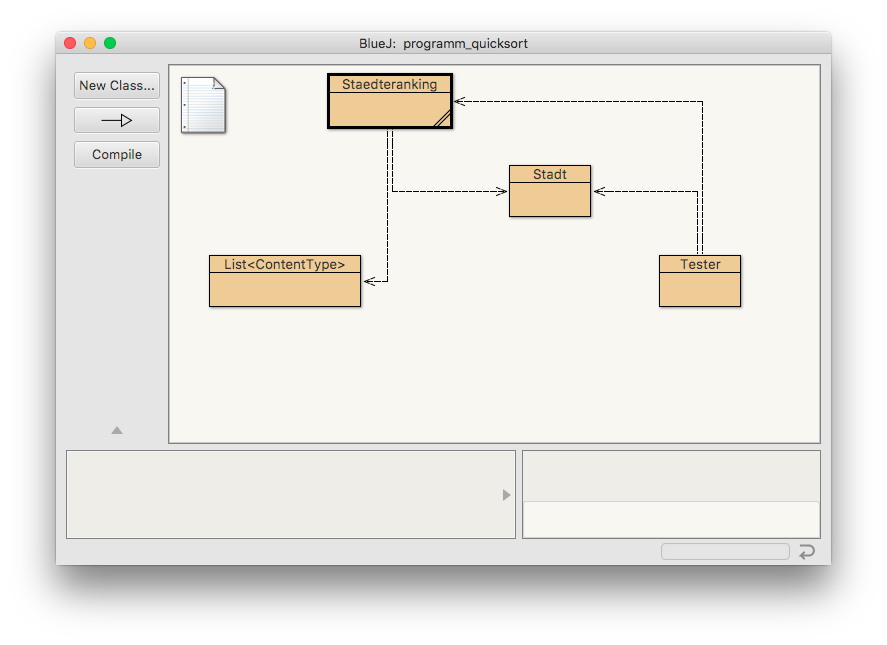
\includegraphics[width=12cm]{bilder/bluej_screenshot.png}
    \caption[Screenshot von BlueJ.]{Der Screenshot zeigt die verwendeten Klassen und ihre Beziehungen in BlueJ.}
    \label{fig:bluejscreenshot}
\end{figure}

Erläuterungen:

\begin{itemize}
    \item \textbf{Die Klasse \javainline{Stadt}}: Objekte dieser Klasse werden von der Klasse \javainline{Staedteranking} in einer Liste verwaltet. Objekte dieser Klasse werden verwendet, um die Städte aus Tabelle~\ref{tabl:staedtekreisborken} zu modelllieren. Eine Stadt zeichnet sich durch einen Namen und eine Einwohnerzahl aus, entsprechende Getter-Methoden ermöglichen den Zugriff auf die Attribute.

    \item \textbf{Die Klasse \javainline{Staedteranking}}: In dieser Klasse werden die Städte in einer als Attribut angelegten Liste von Namen \javainline{rankingliste} verwaltet, welche über den Konstruktor mit Städten (also Objekten der Klasse \javainline{Stadt}) befüllt wird. Ferner gibt es die Möglichkeit, mit der Methode \javainline{neueStadtInsRankingAufnehmen(Stadt pStadt)} eine neue Stadt der Liste hinzuzufügen. Die Klasse stellt außerdem auch die Methoden zum Sortieren  und Ausgeben der Liste bereit.

    \item \textbf{Die Klasse \javainline{Tester}}: Diese Klasse dient zum Testen der Programmierung (ihr Klassendiagramm ist in \Abb\ref{fig:klassendiagramm} nicht aufgeführt). Beim Instanziieren der Klasse wird eine Test-Methode direkt ausgeführt, welche das Städteranking (also die sortierte Liste der Städte) ausgibt.

    \item \textbf{Die Klasse \javainline{List<ContentType>}}: Dies ist die bekannte NRW-Landesklasse. Eine Dokumentation der Klasse findet sich im Anhang (\Seite \pageref{app:javadocliste}).
\end{itemize}





\subsection{Klassendiagramm}
\label{sec:klassendiagramm}
Das Klassendiagramm in Abbildung~\ref{fig:klassendiagramm} zeigt die verwendeten Klassen. Zu beachten ist insbesondere die über das Attribut \javainline{rankingliste} verwaltete Liste an Städten in der Klasse \javainline{Staedteranking}. Die Klasse \javainline{Tester} ist nicht aufgeführt.

\vspace{2em}

\begin{figure}[H]
    \centering
    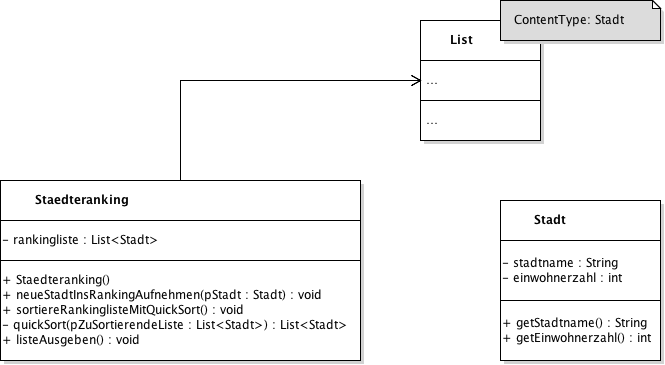
\includegraphics[width=12cm]{bilder/klassendiagramm.png}
    \caption[Klassendiagramm.]{Das Klassendiagramm zum BlueJ-Projekts.}
    \label{fig:klassendiagramm}
\end{figure}





\subsection{Implementation des Quicksort-Algorithmus}
\label{sec:implementationQS}
Im Folgenden wird der Quicksort-Algorithmus unter Verwendung der Landesklasse \javainline{List} implementiert. Zu beachten ist dabei, dass es dafür zwei Methoden in der Klasse \javainline{Staedteranking} gibt. Die private Methode \javainline{private List<Stadt> quickSort(List<Stadt> pZuSortierendeListe)} sortiert dabei die übergebene Liste \javainline{pZuSortierendeListe} (diese Methode wird im Folgenden genauer analysiert). Die Methode \javainline{public void sortiereRankinglisteMitQuickSort()} ruft diese Methode nur auf und veranlasst damit das Sortieren der Rankingliste.

Als Pivotelement wird immer das letzte Element einer Liste gewählt.





\subsubsection{Pseudocode}
\label{sec:pseudocodeQuicksort}
Folgender Pseudocode liegt der Methode \javainline{private List<Stadt> quickSort(List<Stadt> pZuSortierendeListe)} zugrunde (Algorithmus~\ref{algo:qs}). Die sortierte Liste wird am Ende zurückgegeben.

\vspace{1em}

{\footnotesize
\begin{algorithm}[H]
    \DontPrintSemicolon
    
    \KwIn{Liste an Daten (Eingabeliste)}
    \KwOut{Sortierte Liste (Rückgabe der sortierten Liste)}
    
    \BlankLine

    \eIf{Eingabeliste nicht leer}{
        \emph{Deklariere und initialisiere eine leere linke Liste}\;
        \emph{Deklariere und initialisiere eine leere rechte Liste}\;
        \emph{Deklariere und initialisiere eine leere sortierte Liste}\;

        \BlankLine

        \emph{Speichere das letzte Element der Eingabeliste als Pivotelement zwischen}\;
        \emph{Entferne das letzte Element aus der Eingabeliste}\;
        
        \BlankLine

        \emph{Springe an den Anfang der Eingabeliste}\;
        
        \BlankLine

        \While{Eingabeliste nicht leer}{
            \eIf{Aktuelles Element der Eingabeliste kleiner als Pivotelement}{
                \emph{Füge das aktuelle Element der Eingabeliste in die linke Liste ein}\;
                \emph{Entferne das aktuelle Element aus der Eingabeliste}\;
            }
            {
                \emph{Füge das aktuelle Element der Eingabeliste in die rechte Liste ein}\;
                \emph{Entferne das aktuelle Element aus der Eingabeliste}\;
            }
            
            \emph{Springe ein Element in der Eingabeliste weiter}\;
        }

        \emph{Hänge an die sortierte Liste die \textbf{rekursiv} sortierte linke Liste an}\;
        \emph{Hänge an die sortierte Liste das Pivotelement an}\;
        \emph{Hänge an die sortierte Liste die \textbf{rekursiv} sortierte rechte Liste an}\;

        \BlankLine

        \emph{Gib die sortierte Liste zurück}\;
    }
    {
        \emph{Gib nichts zurück}\;
    }

    \caption[Quicksort-Pseudocode (für die Datenstruktur Liste).]{Quicksort auf Listen (allgemeiner Pseudocode).}
    \label{algo:qs}
\end{algorithm}
}

\newpage
\noindent
Es lassen sich also folgende Schritte aus dem Pseudocode ableiten:

\begin{enumerate}
    \item Es wird überprüft, ob die zu sortierende Liste überhaupt Elemente aufweist (falls ja, wird sortiert, falls nein, wird \javainline{null} zurückgegeben).
    
    \item Es werden drei Listen deklariert (\javainline{linkeListe}, \javainline{rechteListe}, \javainline{gebauteListe}).
    
    \item Es werden die drei Listen als leere Listen instanziiert.
    
    \item Es wird an das Ende der zu sortierenden Liste gesprungen.
    
    \item Das Pivotelement wird bestimmt, indem die Stadt in der lokalen Variable Stadt \javainline{pivot} abgespeichert wird.
    
    \item Das Pivotelement wird aus der zu sortierenden Liste entfernt.
    
    \item Es wird an den Anfang der zu sortierenden Liste gesprungen.
    
    \item Die zu sortierende Liste wird komplett durchlaufen und die Elemente der Liste~-- ausgehend von den Einwohnerzahlen der \enquote{Pivotstadt}~-- in die linke bzw. rechte Liste kopiert.
    
    \item An die (noch leere) gebaute Liste wird die rekursiv sortierte linke Liste angehangen.
    
    \item An die gebaute Liste wird die \enquote{Pivotstadt} angehangen.
    
    \item An die gebaute Liste wird die rekursiv sortierte rechte Liste angehangen.
    
    \item Die vollständig sortierte Liste wird zurückgegeben.
\end{enumerate}





\subsubsection{Java-Quelltext}
\label{sec:quelltexterklaerung}
Die öffentliche \javainline{public void sortiereRankinglisteMitQuickSort()} wird zum Sortieren der Rankingliste aufgerufen und ist selbsterklärend (\vgl Quelltext~\ref{lst:methode1oeffentlich}); die Referenz \javainline{rankingliste} wird auf die zurückgegebene Liste gesetzt. Damit wird die unsortierte Rankingliste von der Garbage Collection entfernt, sodass nur noch die sortierte Liste unter der Referenz zu erreichen ist.

\vspace{1em}

\javaexternal[language={Java}, linerange={28-30}, caption={[Öffentliche Methode zum Sortieren der Rankingliste.]{Öffentliche Methode zum Sortieren der Rankingliste. Der Aufruf, die Rankingliste zu sortieren, wird direkt an die eigentliche Sortiermethode wird direkt aufgerufen (\vgl~Quelltext~\ref{lst:methode2privat}). Die Trennung ist notwendig, da die Sortiermethode rekursiv arbeitet.}}, label={lst:methode1oeffentlich}]{quelltexte/programm_quicksort/Staedteranking.java}

Die Methode \javainline{private List<Stadt> quickSort(List<Stadt>  pZuSortierendeListe)} (Quelltext~\ref{lst:methode2privat}) setzt den Pseudocode aus Kapitel~\ref{sec:pseudocodeQuicksort} um. Sie ist privat, da sie nur von der Methode aus Quelltext~\ref{lst:methode1oeffentlich} aufgerufen wird. Außerdem ist zu beachten, dass diese Methode rekursiv arbeitet (und am Ende die sortierte Liste zurückgibt); eine Trennung des Sortierproblems in zwei Methoden ist also notwendig, da die Methode aus Quelltext~\ref{lst:methode1oeffentlich} nichts zurückgibt.

Zu beachten ist, wie die drei Listen deklariert und initialisiert werden und die übergebene Liste mit der \javainline{hasAccess()}-Methode durchlaufen wird. Dieses Vorgehen ist aus dem Unterricht bekannt.

Für den Vergleich einer Stadt mit dem Pivotelement (der Pivotstadt) ist darauf zu achten, dass unbedingt \javainline{pZuSortierendeListe.getContent().getEinwohnerzahl()} aufgerufen wird, um von der Liste auf die aktuelle Stadt und von der aktuellen Stadt auf die Einwohner zugreifen zu können.

Zum Zusammenfügen der linken und rechten Teillisten wird am Ende die Methode \javainline{concat(...)} der Liste verwendet, in deren Parametern auch die rekursiven Aufrufe stattfinden. Um das Pivotelement in der \enquote{Mitte} einzufügen, muss die Methode \javainline{append(...)} verwendet werden, um die Stadt (also das Objekt der Klasse \javainline{Stadt}) an den ersten Teil der sortierten Liste hinten anzuhängen.

\vspace{1em}

\javaexternal[language={Java},linerange={32-105}, caption={Private Methode zum Sortieren einer übergebenen Liste.}, label={lst:methode2privat}]{quelltexte/programm_quicksort/Staedteranking.java}





\subsubsection{Ausgabe}
Das Program gibt die nach Einwohnerzahl sortierte Liste der Städte aus Tabelle~\ref{tabl:staedtekreisborken} in der Konsole aus (Quelltext~\ref{lst:ausgabeKonsole}), wenn die Klasse \javainline{Tester} instanziiert wird. Ein Screenshot ist in Abbildung~\ref{fig:ausgabescreenshot} gegeben (\Seite\pageref{fig:ausgabescreenshot}).

\vspace{1em}

% Java-Quelltext einbinden, Verweis auf Zeilen im Quelltext
\begin{java}[caption={[Ausgabe des Programms in der Konsole.]{Ausgabe in der Konsole. Die Städte liegen nach Einwohnerzahlen sortiert vor -- von Isselburg (\Zeile\ref{lstline:isselburg}) bis Bocholt (\Zeile\ref{lstline:bocholt}).}},label={lst:ausgabeKonsole},escapechar={|}]
Rankingliste:
*************
Isselburg: 10713 |\label{lstline:isselburg}|
Velen: 12989
Gescher: 17253
Rhede: 19165
Stadtlohn: 20367
Vreden: 22561
Ahaus: 39185
Borken: 42509
Gronau: 47671
Bocholt: 71036 |\label{lstline:bocholt}|
\end{java}





\newpage
\section{Fazit}
\label{sec:fazit}
In dieser Facharbeit wurde gezeigt, dass Quicksort ein sehr schneller und leicht zu implementierender Sortieralgorithmus ist. Mit einer Laufzeit von $\mathcal{O}\left(n\log_2{(n)}\right)$ ist er sogar eines der schnellstmöglichen vergleichsbasierten Sortieralgorithmen. Im schlechtesten Fall ist die Laufzeit allerdings quadratisch und damit genauso langsam wie \zB Selectionsort. Da beim randomisierten Quicksort der schlechteste Fall allerdings äußerst unwahrscheinlich ist und in der Praxis eine Datenmenge \idR nicht \emph{komplett} mit Quicksort sortiert wird, kann dieser Nachteil gegenüber anderen Sortieralgorithmen vernachlässigt werden.

\subsection{Blick in die Praxis}
Quicksort existiert in vielen Varianten, die sich in der Wahl des Pivotelements unterscheiden: 

\begin{quote}
Es ist möglich, mit einer Variante von Quicksort auch im schlechtesten Fall eine Zeitkomplexität von $\mathcal{O}\left(n\log_2{(n)}\right)$  zu erreichen (indem als Vergleichselement der Median gewählt wird). Dieses Verfahren ist jedoch im Durchschnitt und im schlechtesten Fall um einen konstanten Faktor langsamer als Heapsort oder Mergesort \textins{\vgl\Kap\ref{sec:ausblick}}; daher ist es für die Praxis nicht interessant.

\hfill\cite{uniflensburgQS}
\end{quote}





\subsection{Ausblick auf andere Algorithmen}
\label{sec:ausblick}

\paragraph{Mergesort}
Ein anderer Sortieralgorithmus, der ebenfalls nach dem Teile-und-Herrsche-Prinzip funktioniert, ist der Mergesort-Algorithmus (\vgl \cite{wikiSortierverfahren}). Bei diesem Verfahren wird beim Zusammensetzen der Teillösungen (\enquote{combine}) die Sortierung erzielt (und nicht durch das geschickte Aufteilen in die Teilprobleme wie beim Quicksort-Algorithmus). 

\paragraph{Heapsort}
Heapsort ist mit einer Laufzeit von $\mathcal{O}\left(n\log_2{(n)}\right)$ genau wie Quicksort ebenfalls optimal (\vgl \cite{wikiSortierverfahren}). Dieses Sortierverfahren verwendet eine besondere Datenstruktur, die als >>Heap<< bezeichnet wird. Ein Heap basiert auf der Datenstruktur >>Baum<<. Auf weitere Ausführungen wird an dieser Stelle verzichtet.





\subsection{Schwierigkeiten beim Bearbeiten der Facharbeit}
\lipsum[3]{}





\newpage
\section{Weitere Informationen}
\label{sec:weitereInfos}
Kapitel~\ref{sec:quellenfacharbeit} gibt ein paar Hinweise, wie die Recherche für die Facharbeit anfangen kann. Es ist sinnvoll, zunächst das Inhaltsverzeichnis der Facharbeit sehr genau auszuarbeiten, bevor mit der \enquote{Schreibarbeit} begonnen wird. Vielleicht ist es auch sinnvoll, Texte erst stichpunktartig vorzuschreiben, um den Umfang und genauen Inhalt eines Kapitels besser abschätzen zu können. Für die Struktur des Inhaltsverzeichnis kann auch ein Blick in die ausgezeichneten Arbeiten des Hans-Riegel-Fachpreises helfen (\Kap\ref{sec:hrfp}).

In Kapitel~\ref{sec:infosLatex} werden Informationen zu \LaTeX{} gegeben. Nützliche Programme für Informatik und Mathematik werden in den Kapiteln~\ref{sec:programmeInformatik} und \ref{sec:programmeMathematik} vorgestellt.   

Sehr gute Facharbeiten können auch am Hans-Riegel-Fachpreis teilnehmen. Mehr Informationen werden in Kapitel~\ref{sec:hrfp} gegeben.





\subsection{Quellenrecherche für die Facharbeit}
\label{sec:quellenfacharbeit}
Ansätze für die Literaturrecherche könnten sein:

\begin{itemize}
    \item Wikipedia-Artikel
    
    \item Quellen des Wikipedia-Artikels (unten auf der Seite)
    
    \item Suchen Sie nach Präsentationen (als PDFs) aus dem universitärem Kontext. Am Ende der Präsentationen finden sich häufig Literaturverweise. 
    
    \item Einige Webseiten \bzw Verlage bieten eine \enquote{Blick ins Buch}-Funktion, wenn ein Buch gefunden ist. So kann man sich einen Überblick über die Inhalte des Buches verschaffen.
    
    \item Einige Bücher sind vielleicht auch auf Google Books zugänglich. \url{https://books.google.com/}
    
    \item Bibliotheken (auch die Schulbibliothek)
\end{itemize}





\subsection{Weitere Informationen zu Latex}
\label{sec:infosLatex}
Folgende Informationen könnten interessant sein:

\begin{itemize}
    \item \textbf{Installation}: Neben dem \LaTeX- \bzw \TeX-System wird ein Editor benötigt, in welchem die \texttt{tex}-Datei bearbeitet und zum PDF-Dokument übersetzt wird. Online finden sich viele Installationsanleitungen für verschiedene Betriebssysteme.
    
    Empfehlenswert sind:
        \begin{itemize}
            \item \textbf{Windows}:
                    \begin{itemize}
                        \item \TeX-System: >>MikTex<<, \url{https://miktex.org/} (oder >>TexLive<<, \url{https://www.tug.org/texlive/})
                        \item Editor: >>TexMaker<<, \url{https://www.xm1math.net/texmaker/}
                    \end{itemize}
    
            \item \textbf{macOS}:
                    \begin{itemize}
                        \item \TeX-System: >>MacTex<<, \url{https://www.tug.org/mactex/}
                        \item Editor: >>TeXShop<<, \url{https://pages.uoregon.edu/koch/texshop/}
                    \end{itemize}
            \item Übersicht und Vergleich verschiedener Editoren (für verschiedene Betriebssysteme): \url{https://en.m.wikipedia.org/wiki/Comparison_of_TeX_editors}
            
            \item Es gibt auch Online-Latex-Editoren (dann ist keine Installation notwendig), \bspw >>Overleaf<<, \url{https://www.overleaf.com/}
        \end{itemize}
    
    \item \textbf{Latex-Einstieg, Erklärungen}:     >>learnlatex.org<<. Lesen Sie unbedingt die ersten Kapitel zum Einstieg, wenn Sie das erste Mal mit Latex arbeiten.
        
    \item \textbf{Latex-Befehl für ein Zeichen vergessen?}: >>Detexify<<. Man kann das gesuchte Zeichen mit der Maus malen und die Webseite gibt einen passenden Latex-Befehl aus. \url{http://detexify.kirelabs.org/classify.html}
    
    \item \textbf{Mathematischer Textsatz}: >>Wikipedia-Hilfe<<. Setzen von Integralen, Summen, Reihen, Matrizen \etc \url{https://de.wikipedia.org/wiki/Hilfe:TeX}
    
    \item \textbf{Wissenschaftliche Arbeiten als Vorlage}: Im Internet finden sich viele Latex-Einstiegsbeispiele und Vorlagen für Bachelor-, Master- und Diplomarbeiten. Es empfiehlt sich, gezielt nach PDF-Dokumenten zu suchen.
    
    \item \textbf{Grafiken}: >>LatexDraw<<. Grafiken selbst gestalten und Latex-kompatibel exportierten (für die PSPicture-Umgebung von Latex). \url{http://latexdraw.sourceforge.net/}
    
    \item \textbf{Grafiken, Graphen}: Möchte man Grafiken selbst erstellen, empfiehlt sich das Latex-Paket >>TikZ<<. TikZ braucht aber etwas Eingewöhnung -- andere Programme sind da häufig einfacher (bspw. LatexDraw, \sieheoben). Eine kleine, erste Übersicht findet man unter \url{https://www.overleaf.com/learn/latex/TikZ_package} und \url{https://en.wikibooks.org/wiki/LaTeX/PGF/TikZ}.
    
    \item \textbf{Bilder und Grafiken}: Bilder und Grafiken sollten wenn möglich als PDF exportiert werden (Vektorgrafik). Wenn dies nicht möglich ist, sind \texttt{eps}-Dateien den üblichen Bild-Dateien (\texttt{png}, \texttt{jpg}) vorzuziehen, da dies ebenfalls Vektorgrafiken sind.
    
    \item \textbf{Dokumentation von Paketen}: >>CTAN<<. Zu jedem Paket, welches in der Präambel des Dokuments geladen wurde, findet sich auf CTAN eine Dokumentation. Diese wird aber häufig sehr schnell sehr umfangreich und detailreich, kann aber für sehr spezielle Fragen einen Blick wert sein. \url{http://www.ctan.org/tex-archive/macros/latex/contrib/}
    
    \item \textbf{Hilfeforum}: >>Tex.Stackexchange<<, \url{https://tex.stackexchange.com/}
    
    \item \textbf{Verweise auflösen}: Vergessen Sie nicht, Ihr Dokument mehrfach zu übersetzen, um alle Verweise aufzulösen (damit alle >>\textbf{??}<< aufgelöst werden). Das Paket \texttt{refcheck} (s.~Präambel dieses Dokuments) gibt Hinweise auf kaputte Verweise.
\end{itemize}




\subsection{Programme für Informatik}
\label{sec:programmeInformatik}
Einige Dienste setzen Accounts voraus, andere sind ohne Account nutzbar. Zum Teil sind Grafiken \etc nicht ohne Account zu speichern oder zu exportieren. In jedem Fall sollte man erst ein bisschen ausprobieren und verschiedene Dienste miteinander vergleichen (immer vor dem Hintergrund, später noch Änderungen vorzunehmen!), bevor man viel Zeit und Mühe in Grafiken investiert.

\begin{itemize}
    \item \textbf{Zeichnungen, Grafiken, Infografiken}: >>Draw.io<<. Sehr umfangreich und mächtig -- es gibt viele Vorlagen (\zT auch UML-konform). \url{https://www.draw.io}
    
    \item \textbf{Zeichnungen, Sequenzdiagramme, Graphen}: >>HackMD<<. Sehr umfangreich und nach kurzer Einarbeitung einfach zu bedienen. \url{https://hackmd.io}, Feature-Übersicht: \url{https://hackmd.io/features?both}
    
    \item \textbf{ER-Diagramme}: >>ERDplus<<, \url{https://erdplus.com/}
    
    \item \textbf{Graphen, Automaten, Formale Sprachen}: >>FLACI<<. Kann auch DEAs, NEAs und Kellerautomaten simulieren. \url{https://flaci.com/home/}
    
    \item \textbf{Struktogramme}: >>Struktogrammeditor<<, \url{https://whiledo.de/index.php?p=struktogrammeditor}
    
    \item \textbf{Klassendiagramme, Objektdiagramme, UML-Diagramme}: >>Violet UML<<. Abbildung~\ref{fig:klassendiagramm} wurde mit Violet UML erstellt. \url{http://alexdp.free.fr/violetumleditor/page.php}
    
    \item \textbf{UML-Diagramme}: >>Dia<<. Professioneller als Violet UML (\so). \url{http://dia-installer.de/} 
    
    \item \textbf{UML-Diagramme, ER-Diagramme}: >>yEd<<. Professioneller, aber auch umständlicher als Violet UML. \url{https://www.yworks.com/products/yed}. 
    
    Dieses Programm wird auch genutzt, um die Klassen-, Objekt- und ER-Diagramme für die Abiturprüfungen zu erstellen. Im Lehrplannavigator Informatik gibt es auch die NRW-spezifische Symbole und NRW-Beispiel-Diagramme für yED zum Download, \vgl \enquote{Weiterführende Quellen} unter \url{https://www.schulentwicklung.nrw.de/lehrplaene/lehrplannavigator-s-ii/gymnasiale-oberstufe/informatik/hinweise-und-beispiele/index.html} 
    
    \item \textbf{Sequenzdiagramme}: >>js-sequence-diagrams<<, \url{https://bramp.github.io/js-sequence-diagrams/} und >>WebSequenceDiagrams<<, \url{https://www.websequencediagrams.com/}
    
    \item \textbf{Java-Nachschlagewerk}: >>Java ist auch eine Insel<< von C. \textsc{Ullenboom}, \url{http://openbook.rheinwerk-verlag.de/javainsel/}
    
    \item \textbf{Visualisierungen von Algorithmen}: >>Visualgo<<. Nachschlagewerk und sehr gute Visualisierung. Hat auch die Möglichkeit, eigene Beispiele auszuprobieren. \url{https://visualgo.net/de}
    
    \item \textbf{Landesklassen}: Lehrplannavigator Informatik (Kapitel \enquote{Grundlegende Materialien und Dokumentationen für den Unterricht und für das Zentralabitur}), \url{https://www.schulentwicklung.nrw.de/lehrplaene/lehrplannavigator-s-ii/gymnasiale-oberstufe/informatik/hinweise-und-beispiele/index.html}. 
    
    Dort ist ebenfalls die Dokumentation der Landesklassen verlinkt (GK- und LK-Variante). GK:  \url{https://www.schulentwicklung.nrw.de/lehrplaene/upload/klp_SII/if/MaterialZABI/2017-11-28_Dokumentation_GK_ab_Abitur_2018.pdf}, LK: \url{https://www.schulentwicklung.nrw.de/lehrplaene/upload/klp_SII/if/MaterialZABI/2017-11-28_Dokumentation_LK_ab_Abitur_2018.pdf}
    
    \item \textbf{Java-Entwicklungsumgebung für die Schule}: >>BlueJ<<, \url{https://www.bluej.org/}
    
    \item \textbf{Umfangreiche Java-Entwicklungsumgebung}: >>NetBeans<<. Diese IDE halte ich am ehesten für Einsteiger geeignet. \url{https://netbeans.org/}
    
    \item \textbf{Profi-Java-Entwicklungsumgebung}: >>Eclipse<<, \url{https://www.eclipse.org/}
    
    \item \textbf{Profi-Java-Entwicklungsumgebung}: >>IntelliJ IDEA<<, \url{https://www.jetbrains.com/idea/}
\end{itemize}





\subsection{Programme für Mathematik}
\label{sec:programmeMathematik}
Folgende Programme und Dienste können für Facharbeiten im Fach Mathematik interessant sein.

\begin{itemize}
    \item \textbf{Alleskönner, CAS}: >>Wolfram Alpha<<. Gewissermaßen eine Suchmaschine für Lösungen zu mathematischen Probleme. Ergebnisse lassen sich als Latex-Formelcode kopieren. Kauft man die App, werden auch Lösungswege angezeigt. \url{https://www.wolframalpha.com/}

    \item \textbf{Mini-CAS}: >>Eigenmath<<. Rechnet symbolisch (und nicht algebraisch!) und programmierbar. \url{http://www.eigenmath.org/}

    \item \textbf{Graphen, Visualisierungen, CAS}: >>GeoGebra<<. Graphen lassen sich Latex-kompatibel exportieren (für PSPicture oder TikZ). Alternativ empfiehlt sich der Export als PDF. \url{https://www.geogebra.org/}

    \item \textbf{Formeln von Wikipedia}: Möchte man Formeln von Wikipedia kopieren (und nicht abschreiben), kann man sich über die Funktion \enquote{Quelltext bearbeiten} eines Abschnitts \bzw Artikels den Quelltext (und damit auch die Formel in Latex-Notation!) anzeigen lassen und kopieren.
\end{itemize}





\subsection{Hans-Riegel-Fachpreis}
\label{sec:hrfp}
Gute Facharbeiten aus dem MINT-Bereich können bei der Hans-Riegel-Stiftung eingereicht werden (die Arbeiten sollten über die Schule eingereicht werden). Informationen (und auch ausgezeichnete Arbeiten) können auf der Webseite des Dr.-Hans-Riegel-Fachpreises eingesehen werden. Es gibt Geldpreise zu gewinnen. Der \textbf{Einsendeschluss} ist zu beachten (\idR 01. Mai eines jeden Jahres).

Die Preisverleihung findet für Schulen unseres Kreises traditionell im Schloss Münster statt. Die Anzahl der eingereichten Arbeiten war in den letzten Jahren vergleichsweise gering, sodass die Chancen auf einen Gewinn insgesamt gut sind (eine entsprechende Facharbeit natürlich vorausgesetzt).

\vspace{2em}

\noindent
\textbf{Informationen zum Wettbewerb}: 
\begin{center}
    \url{https://www.hans-riegel-fachpreise.com/wettbewerb/}
\end{center}

\vspace{1em}

\noindent
\textbf{Ausgezeichnete Facharbeiten}:

\begin{center}
    \url{https://www.hans-riegel-fachpreise.com/ausgezeichnete-arbeiten/}
\end{center}

\vspace{1em}

\noindent
\textbf{Kooperation WWU Münster}:

\begin{center}
    \url{https://www.hans-riegel-fachpreise.com/universitaeten/westfaelische-wilhelms-universitaet-muenster/}
\end{center}





\newpage
\phantomsection
\addcontentsline{toc}{section}{\protect\numberline{}{\bibname}}
\renewcommand{\refname}{\bibname}
\begin{thebibliography}{50}

    \bibitem[Hoare 1962]{hoare} C. A. R. \textsc{Hoare} (1962): \emph{Quicksort}. Computer Journal, Vol. 5, 1, \Seite 10--15.
    
    \bibitem[IDEA]{ideaBauanleitung} S. P. \textsc{Fekete}, S. \textsc{Morr} (2018): \emph{KVICK SÖRT}. \url{https://idea-instructions.com/quick-sort/}, aufgerufen am 02.04.2020.

    \bibitem[Kempe Löhr 2015]{schoeninghQ1Q2} T. \textsc{Kempe},  A. \textsc{Löhr} (Hrsg.) (2015): \emph{Informatik~--~Lehrwerk für die gymnasiale Oberstufe~--~Neubearbeitung. Schülerband 2.} Schöningh-Verlag. Paderborn.
    
    \bibitem[Khan 2020]{khanqslaufzeit} Khan Academy (2020): \emph{Analyse von Quicksort}. \url{https://de.khanacademy.org/computing/computer-science/algorithms/quick-sort/a/analysis-of-quicksort}, aufgerufen am 08.04.2020.
    
    \bibitem[Lang 2018]{uniflensburgQS} H. W. \textsc{Lang} (2018): \emph{Quicksort}. \url{https://www.inf.hs-flensburg.de/lang/algorithmen/sortieren/quick/quick.htm}, aufgerufen am 07.04.2020.
    
    \bibitem[Lang DuC]{uniflensburgDuC} H. W. \textsc{Lang} (unbekanntes Jahr): \emph{Divide-and-Conquer-Prinzip}. \url{https://www.inf.hs-flensburg.de/lang/glossar/divconq.htm}, aufgerufen am 07.04.2020.
    
    \bibitem[LPN IF Doku GK]{lehrplannavigatorIFDokuGK} Qualitäts- und UnterstützungsAgentur -- Landesinstitut für Schule (2020): \emph{Dokumentation für den Grundkurs}. \url{https://www.schulentwicklung.nrw.de/lehrplaene/upload/klp_SII/if/MaterialZABI/2017-11-28_Dokumentation_GK_ab_Abitur_2018.pdf}, aufgerufen am 07.04.2020.
    
    \bibitem[LPN IF]{lehrplannavigatorIF} Qualitäts- und UnterstützungsAgentur -- Landesinstitut für Schule (2020): \emph{Hinweise und Beispiele zur standardorientierten Unterrichtsentwicklung im Fach Informatik}. \url{https://www.schulentwicklung.nrw.de/lehrplaene/lehrplannavigator-s-ii/gymnasiale-oberstufe/informatik/hinweise-und-beispiele/hinweise-und-beispiele.html}, aufgerufen am 07.04.2020.
    
    \bibitem[VisuAlgo]{visualgoQS} Dr.\,S. \textsc{Halim}, Dr.\,F. \textsc{Halim} (2020): \emph{VisuAlgo.net}. \url{https://visualgo.net/de/sorting}, aufgerufen am 04.04.2020.
    
    \bibitem[Wiki Hoare]{wikiHoare} Wikipedia (2019): \emph{Tony Hoare}. \url{https://de.wikipedia.org/wiki/Tony_Hoare}, Stand 20.03.2019, aufgerufen am 07.04.2020.
    
    \bibitem[Wiki QS]{wikiQS} Wikipedia (2020): \emph{Quicksort}. \url{https://de.wikipedia.org/wiki/Quicksort}, Stand 17.03.2020, aufgerufen am 08.04.2020.
    
    \bibitem[Wiki SortVerf]{wikiSortierverfahren} Wikipedia (2020): \emph{Sortierverfahren}. \url{https://de.wikipedia.org/wiki/Sortierverfahren}, Stand 07.02.2020, aufgerufen am 07.04.2020.
    
    \bibitem[Wiki Stab]{wikiStabilitaet} Wikipedia (2019): \emph{Stabilität (Sortierverfahren)}. \url{https://de.wikipedia.org/wiki/Stabilit\%C3\%A4t_(Sortierverfahren)}, Stand 12.10.2019, aufgerufen am 06.04.2020.

\end{thebibliography}





\newpage
\phantomsection
\addcontentsline{toc}{section}{\protect\numberline{}{\listfigurename}}
\listoffigures





\newpage
\phantomsection
\addcontentsline{toc}{section}{\protect\numberline{}{\listtablename}}
\listoftables





\newpage
\phantomsection
\addcontentsline{toc}{section}{\protect\numberline{}{\listalgorithmcfname}}
\listofalgorithms





\newpage
\phantomsection
\addcontentsline{toc}{section}{\protect\numberline{}{\lstlistlistingname}}
\lstlistoflistings





\newpage
\section*{Anhang}
\addcontentsline{toc}{section}{\protect\numberline{}Anhang}
Der Anhang gliedert sich in:

\begin{enumerate}[label={\alph*)}]
    \item Dokumentation der Landesklasse \javainline{List} (\Seite~\pageref{app:javadocliste})
    \item Hinweise zum Starten des Programms (\Seite~\pageref{app:hinweiseprogrammstart}, \cite{lehrplannavigatorIFDokuGK})
\end{enumerate}

\includepdf[pages={12}, pagecommand={\phantomsection\label{app:javadocliste}\thispagestyle{empty}}]{anhang/2017-11-28_Dokumentation_GK_ab_Abitur_2018.pdf}

\includepdf[pages={13}, pagecommand={\thispagestyle{empty}}]{anhang/2017-11-28_Dokumentation_GK_ab_Abitur_2018.pdf}





\newpage
\section*{Hinweise zum Starten des Programms}
\label{app:hinweiseprogrammstart}
Das Projekt wird wie gewohnt über die \texttt{package.bluej} geöffnet. Wenn die Klasse \javainline{Tester} instanziiert wird, wird über den Konstruktor die Rankingliste in der Klasse \javainline{Staedteranking} mit den Städten aus Tabelle~\ref{tabl:staedtekreisborken} befüllt. Anschließend wird direkt die Testmethode \javainline{public void testeDenQuickSortAlgorithmus()} ausgeführt. Es wird die Ausgabe wie in Abbildung~\ref{fig:ausgabescreenshot} erzeugt.

\begin{figure}[H]
\centering
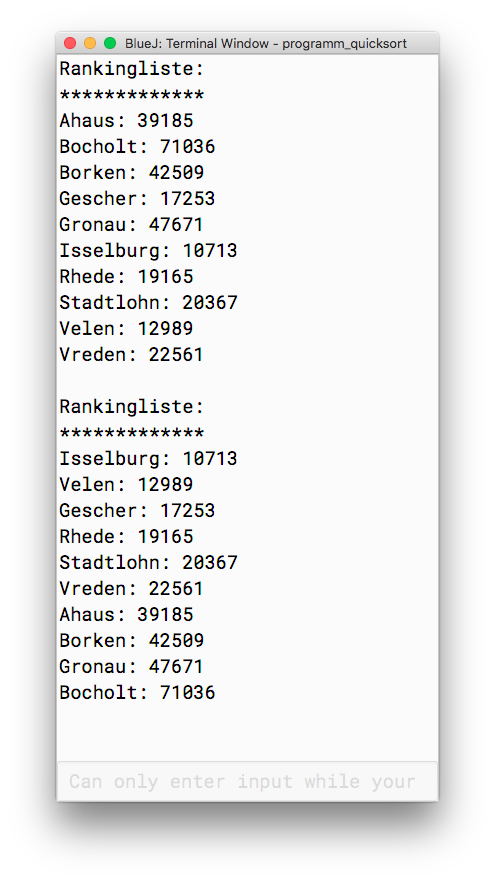
\includegraphics[width=8cm]{bilder/ausgabe_screenshot.png}
\caption[Ausgabe der sortierten Rankingliste.]{Ausgabe des Projekts beim Instanziieren der Testklasse. Die anfänglich nach Namen sortierten Städte (oben) wurden nach Einwohnerzahlen sortiert (unten).}
\label{fig:ausgabescreenshot}
\end{figure}





\newpage
\section*{Selbstständigkeitserklärung}
\addcontentsline{toc}{section}{\protect\numberline{}Selbstständigkeitserklärung}

\emph{Ich erkläre, dass ich die Facharbeit ohne fremde Hilfe angefertigt habe und nur die im Literaturverzeichnis angefügten Quellen und Hilfsmittel benutzt habe. Insbesondere versichere ich, dass ich alle wörtlichen und sinngemäßen Übernahmen aus anderen Werken als solche kenntlich gemacht habe.}

\vspace{2cm}

\noindent
\begin{tabular}{p{5cm}p{1.5cm}p{5cm}}
    \hspace{6cm}  &  &  \hspace{6cm}\\
    \cline{1-1}         \cline{3-3}
    Ort, Datum    &  &  Unterschrift
\end{tabular}





\end{document}